
\documentclass[12pt]{article}

\usepackage{sbc-template}

\usepackage{hyperref}
\hypersetup{
    colorlinks=true,
    linkcolor=blue,
    filecolor=magenta,      
    urlcolor= blue,
    bookmarks=true,
    pdfpagemode=FullScreen,
}


\usepackage{url}

\usepackage{graphicx,url}
\usepackage{amsmath}
\usepackage[brazil]{babel}   
\usepackage[utf8]{inputenc}  
\usepackage{units}
\usepackage{fancyhdr}

\usepackage{indentfirst}
\usepackage[inline]{enumitem}
\pagestyle{fancy}

\fancyhead[L]{ }
\fancyhead[R]{ }

%\chead{\begin{picture}(3,3) \put(-230,-15) {\includegraphics%[width=16cm, height=2.8cm, keepaspectratio=false]{logoSIRC.png}} \end{picture}}
\renewcommand{\headrulewidth}{0pt}
\sloppy
\begin{document} 


\title{Relatório técnico sobre o avanço da pandemia causada pelo vírus SARS-CoV-2 na cidade de Dourados - MS:\\ Análise de dados, comparações de Cenários e modelo preditivo}

\author{Fernando Ferraz Ribeiro\inst{1}, Marco Aurélio Boselli\inst{2},\\ Everaldo Freitas Guedes\inst{3}, Fernanda Vasques Ferreira\inst{4}}
  

 

\address{Universidade Federal da Bahia -- Faculdade de Arquitetura -- LCAD
  (UFBA)\\
  Salvador, BA -- Brasil
\nextinstitute
  Universidade Federal de Uberlândia  -- Instituto de Física (UFU)\\
  Uberlândia, MG -- Brasil 
\nextinstitute
  Bacharel em Estatística, Doutor e Mestre em \\Modelagem Computacional Aplicada à Tecnologia Industrial\\
  Salvador, BA -- Brasil
\nextinstitute
  Universidade Federal do Oeste da Bahia (UFOB)\\
  Santa Maria da Vitória, BA -- Brasil
  \email{fernando.ribeiro@ufba.br, maboselli@gmail.br, }\email{efgestatistico@gmail.com,
  fernanda.jornalista82@gmail.com}
}


\maketitle

\begin{abstract}

  This report presents a study on the progress of the pandemic caused by the SARS-CoV2 virus in the municipality of Dourados - MS. For this purpose, the database provided by the Ministry of Health was used. The report presents a descriptive analysis of the data available in that database. A comparison is presented with the cases diagnosed in other municipalities in the same state and with data from the city of Manaus - AM, used as a reference in an emblematic case of the advance of the pandemic in Brazil. In the end, a predictive model adapted from DELPHI, developed by a research team linked to the \ textit {Massachusetts Institute of Technology} (MIT), is used as an instrument to visualize the future scenario in which the current trends of progress are maintained and confirmed.

\end{abstract}
     
\begin{resumo} 
  Este relatório apresenta um estudo sobre o avanço da pandemia causada pelo vírus SARS-CoV2 no município de Dourados - MS. Para tanto, foi utilizada a base de dados fornecida pelo Ministério da Saúde. O relatório apresenta uma análise descritiva dos dados disponíveis na referida base. É apresentada uma comparação com os casos diagnosticados em outros municípios do mesmo estado e com os dados da cidade de Manaus - AM, utilizado como referência de um caso emblemático do avanço da pandemia no Brasil. Ao fim, um modelo preditivo adaptado do DELPHI, desenvolvido por uma equipe de pesquisa vinculada ao \textit{Massachusetts Institute of Technology} (MIT), é utilizado como instrumento de visualização do cenário futuro em que as atuais tendências de avanço sejam mantidas e confirmadas.
\end{resumo}


\section{Introdução}

O avanço da pandemia da Covid-19, causada pelo vírus SARS-CoV-2, tem se apresentado como o mais importante desafio do tempo presente. Autoridades políticas, cientistas e a sociedade buscam estabelecer planos de enfrentamento com o intuito de minimizar os impactos, direta ou indiretamente ligados à propagação da doença. De acordo com a \textit{Johns Hopkins University}, uma das principais fontes de dados mundiais sobre o tema, o número de casos confirmados no mundo já ultrapassa os 9 milhões (em 23/06/2020).

A adequada coleta e análise dos dados relativos à pandemia tem sido uma importante ferramenta no enfrentamento da crise sanitária da Covid-19, sendo usada para direcionar ações, recursos e informações em todas as esferas da sociedade, na busca de alternativas e soluções para a redução de dados e orientação na tomada de decisões neste contexto pandêmico.

\begin{figure}[!htb]
  \centering
  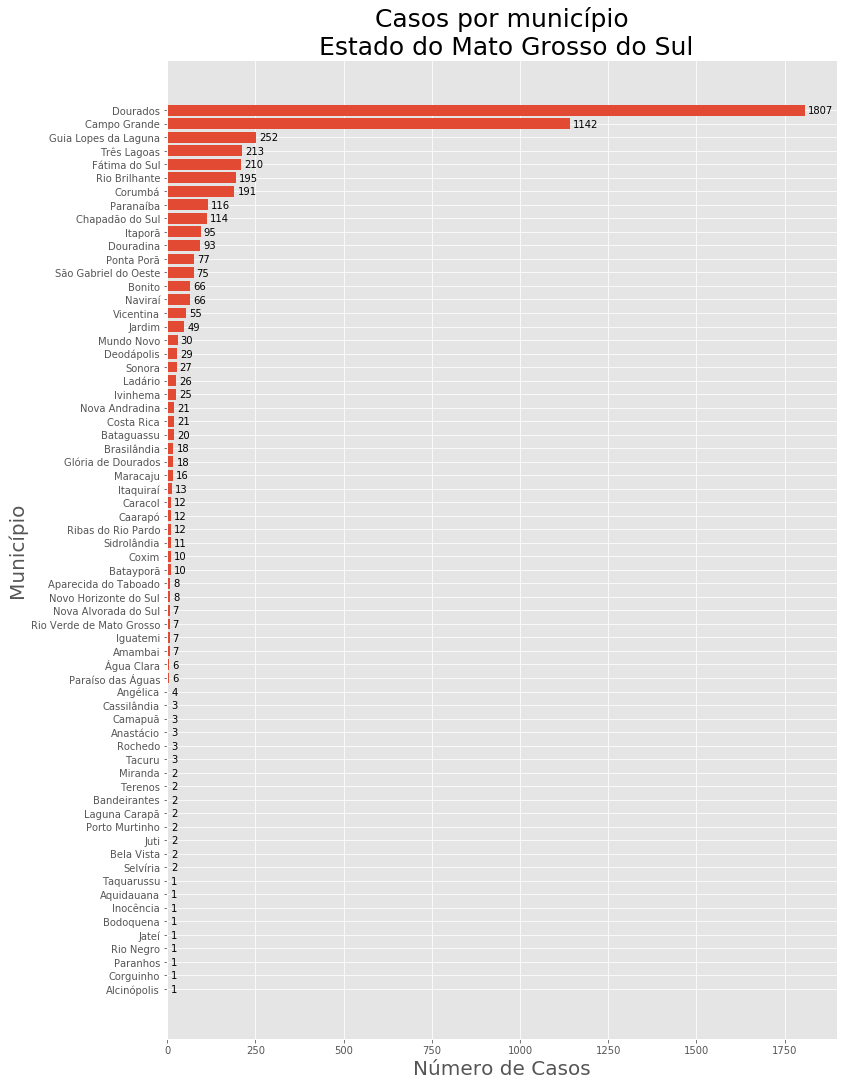
\includegraphics[width=1\textwidth]{figs/casos_por_municipio.png}
  \caption{Número de casos diagnosticados por município (MS)}
  \label{fig:casosMuni}
  \end{figure}

No presente trabalho, uma análise dos dados da cidade de Dourados - MS é apresentada. A situação da cidade é comparada com os demais municípios do estado e a curva de crescimento registrada na referida cidade é comparada com a curva registrada na cidade de Manaus - AM. Em seguida os dados são utilizados para alimentar um modelo preditivo baseado no DELPHI, desenvolvido por uma equipe de pesquisadores ligada ao MIT. Na conclusão, os resultados obtidos são analisados com o objetivo de embasar a tomada de decisões.

\section{Metodologia}\label{sec:met}

Mesmo sob a alardeada interiorização da pandemia no Brasil, o caso do município de Dourados - MS chama a atenção pelo fato de, mesmo com uma população equivalente à \(\nicefrac{1}{4}\) da população de Campo Grande, apresenta um número total de casos diagnosticados aproximadamente 50\% maior do que os registrados na capital.

A fonte de dados utilizada na elaboração deste relatório foi obtida no portal \textbf{CORONAVÍRUS BRASIL}\cite{minsaude}, em que as informações oficiais do Ministério da Saúde sobre a pandemia são disponibilizadas. Os dados usados nas análises como número de casos (acumulados e novos casos) e sobre a população de cada município foram extraídos desta base (até o dia 23/06/2020). 

A partir destas informações, foram comparados o número de casos e a população dos diferentes municípios do estado. Os dados estão representadas em forma de diagramas e mapas (dados geoespaciais) procurando entender como está a distribuição de casos nas diversas regiões do estado. A curva de crescimento dos casos do município foi comparada com a curva do município de Manaus - AM. Nossa análise buscou compreender o quanto o avanço dos casos de contaminação da Covid-19 em Dourados - MS se aproxima do caso emblemático capital do Amazonas.

\begin{figure}[!htb]
  \centering
  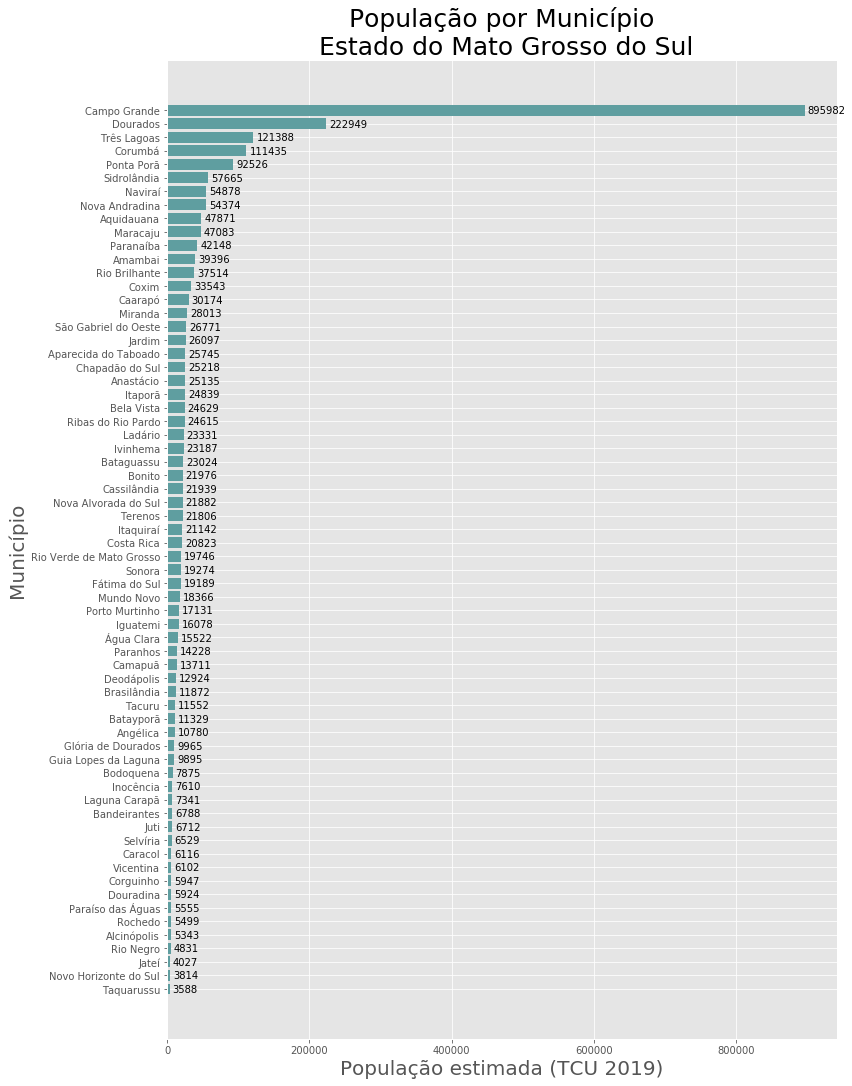
\includegraphics[width=1\textwidth]{figs/pop_por_municipio.png}
  \caption{População por município (MS)}
  \label{fig:popuMuniMS}
  \end{figure}

  Estratégias de visualização de dados e ajuste de polinômios foram utilizadas para ilustrar e entender o caso em estudo. Após essas análises, os dados foram tratados e submetidos ao modelo preditivo escolhido. Ao fim, os resultados são apresentados.

\begin{figure}[!htb]
  \centering
  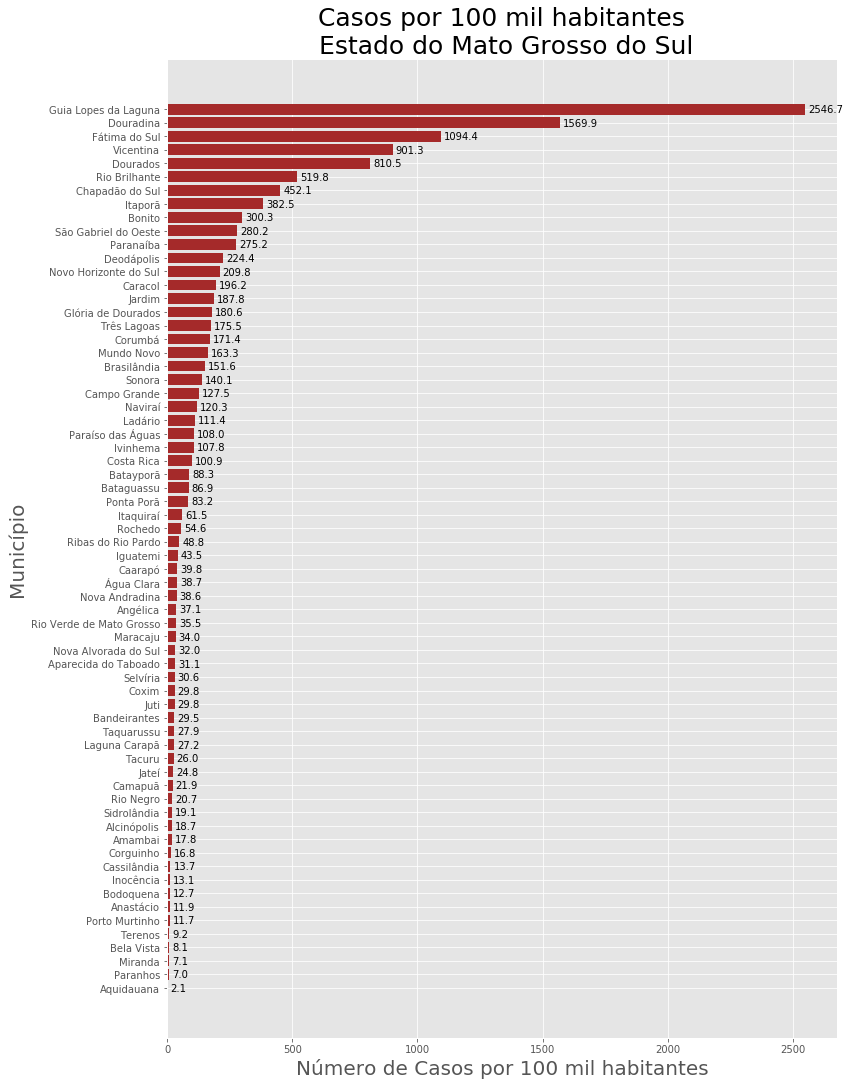
\includegraphics[width=1\textwidth]{figs/casos_100_mil_por_municipio.png}
  \caption{Número de casos por 100 mil habitantes em cada município (MS) extraídos do boletim epidemiológico do dia 21/06/2020}
  \label{fig:casosMuni100k}
  \end{figure}

\section{Análise de Dados}\label{sec:dados}

As Figuras~\ref{fig:casosMuni} e~\ref{fig:popuMuniMS} confirmam as informações sobre a  maior incidência de casos em Dourados do que na capital e mostra que o município está em primeiro lugar em número de casos, sendo o segundo em população do estado.

Já em números relativos, a Figura~\ref{fig:casosMuni100k} indica os casos confirmados por 100 mil habitantes e mostra que a cidade objeto deste estudo está em quinto lugar. As cidades que aparecem nas primeiras posições da lista: Guia Lopes da Laguna, Douradina, Fátima do Sul e Vicentina, pela ordem, têm populações muito inferiores, respectivamente 9.895, 5.924, 19.189 e 6.102 habitantes. A de maior população dentre elas - Guia Lopes da Laguna - apresenta menos de \(\nicefrac{1}{10}\) da população de Dourados. Além de indicar as cidades supracitadas, com os maiores números relativos à população, conforme conforme \ref{fig:casosMuni100k}, as mesmas também aparecem nas primeiras posições na lista das cidades com os maiores em número de casos totais, conforme Figura~\ref{fig:casosMuni}.

\subsection{Comparação da evolução de casos: Dourados, Campo Grande e Mato Grosso do Sul}\label{ssec:DouCGMS}

\begin{figure}[!htb]
  \centering
  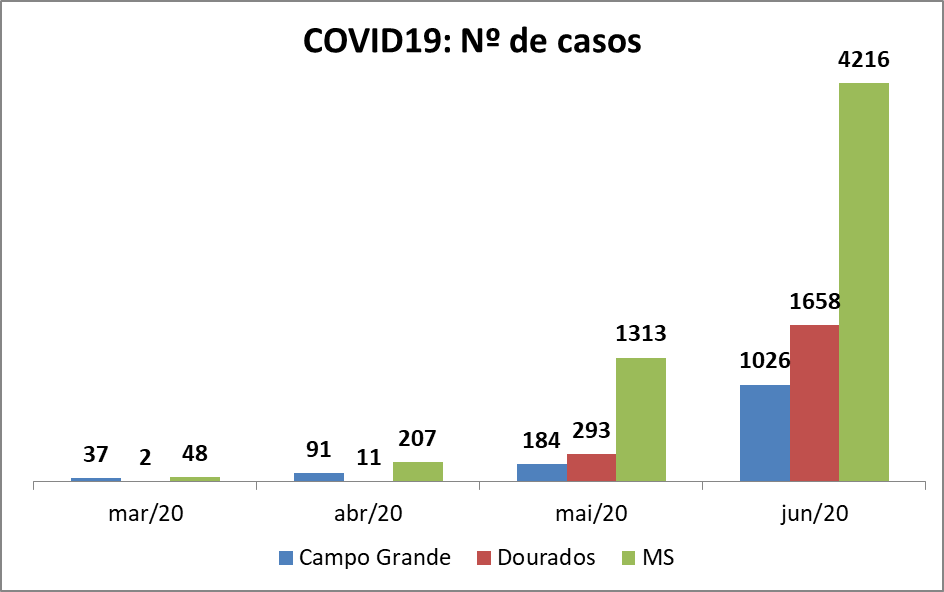
\includegraphics[width=.5\textwidth]{figs/douCGMS01.png}
  \caption{Número de casos}
  \label{fig:douCGMScasos}
  \end{figure}


A Covid-19 evolui de maneira acelerada em Mato Grosso do Sul. Até 23/6/2020 foram registrados 5784 casos com 55 mortes. Mais da metade dos casos da doença está concentrada nos municípios Campo Grande (23,1\%) e Dourados (34,0\%), que totalizam 57,1\% dos casos da doença, conforme Figura~\ref{fig:douCGMScasos}.


Em comparação com a capital do estado, desde os primeiros registros da Pandemia, Dourados tem apresentando as maiores taxas de crescimento mensal em comparação com o mês anterior. A Figura~\ref{fig:douCGMStaxa} mostra que, no mês de Maio o número de infectados cresceu 2563,6\% em relação a abril, já  em  Junho, essa taxa alcança 465,9\%.

\begin{figure}[!htb]
  \centering
  \includegraphics[width=.5
  \textwidth]{figs/douCGMS02.png}
  \caption{Taxa de crescimento do número de casos em relação ao mês anterior}
  \label{fig:douCGMStaxa}
  \end{figure}

\subsection{Dados Geoespaciais}\label{ssec:geo}

O aspecto geográfico é de grande impacto na análise de dados de fenômenos complexos com as características da pandemia provocada pela Covid-19. Os estados, cidades, até mesmo subdivisões menores do espaço como bairros e localidades ou maiores como países e continentes não delimitam populações estanques e incomunicáveis. Entender as dinâmicas de deslocamento das pessoas é fundamental para rastrear os caminhos que o vírus percorreu, mas também para estabelecer estratégias de combate eficazes.

\begin{figure}[!htb]
  \centering
  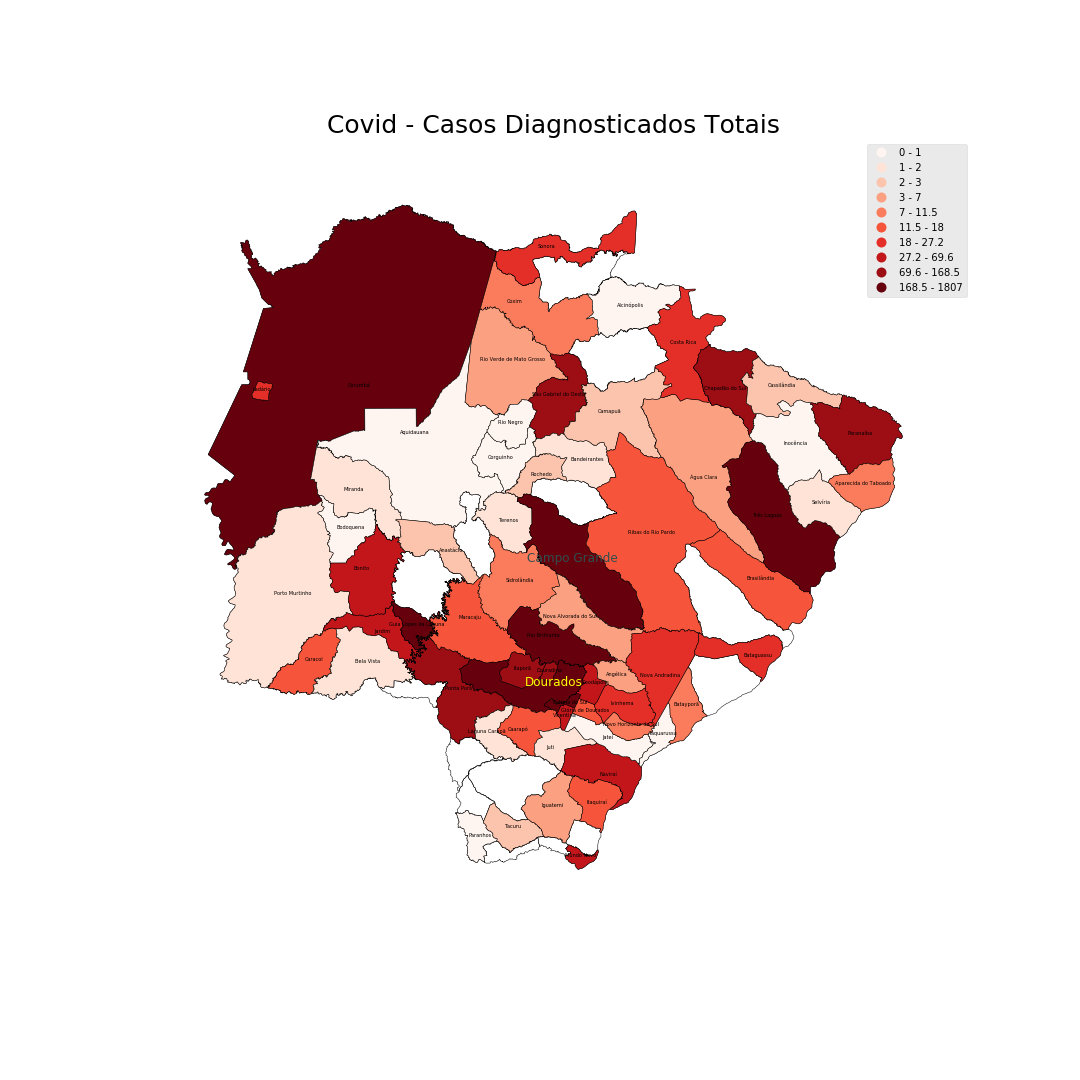
\includegraphics[width=1\textwidth]{figs/mapa_casos_registrados.png}
  \caption{Mapa de casos diagnosticados por município (MS)}
  \label{fig:mapaCasos}
  \end{figure}

Dois mapas foram utilizados para visualizar o cenário atual do estado: um que mostra os municípios com maior incidência de casos totais (Fig.~\ref{fig:mapaCasos}) e outro que mostra a incidência por cem mil habitantes (Fig.~\ref{fig:mapa100K}). Tanto o município de Dourados, quanto seu entorno aparecem em destaque em ambos os mapas.

\begin{figure}[!htb]
    \centering
    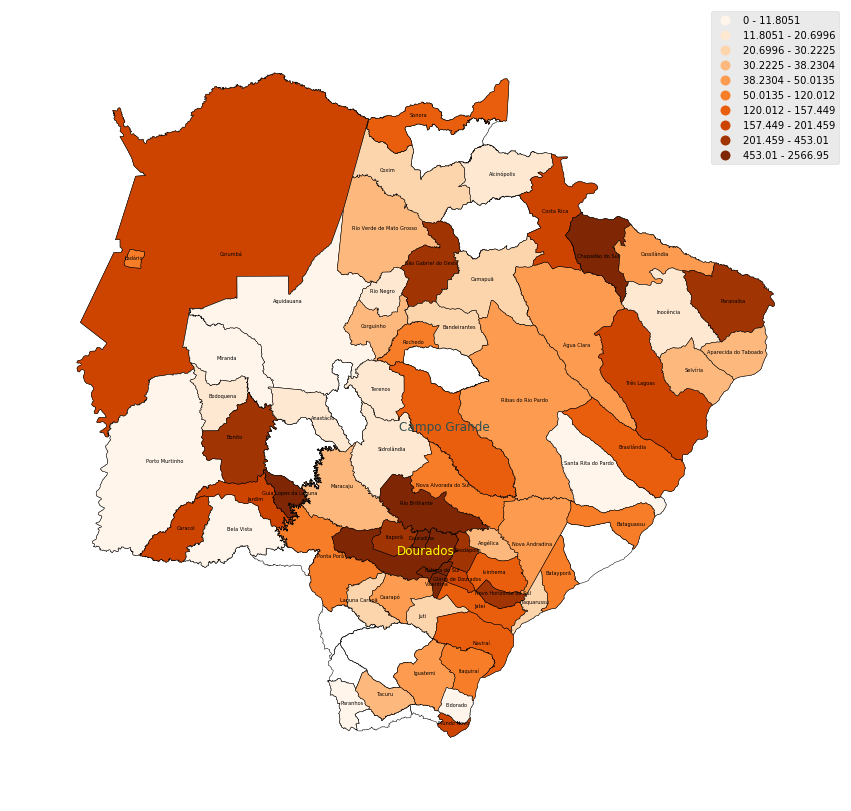
\includegraphics[width=1\textwidth]{figs/mapa_casos_100_mil.png}
    \caption{Número de casos diagnosticados por 100 mil habitantes em cada município (MS)}
    \label{fig:mapa100K}
    \end{figure}
  
Das quatro cidades que apresentam maior número de casos por 100 mil habitantes (Fig.~\ref{fig:casosMuni100k}) apenas Guia Lopes da Laguna não faz fronteira com o município objeto deste estudo. Considerando as dez cidades com maior número de casos por 100 mil habitantes, seis delas fazem divisa com Dourados, que figura em quinto lugar Dessa lista. Douradina está em segundo, Fátima do Sul em terceiro, Vicentina em quarto, Rio Brilhante em sexto, Itaporã em oitavo e Deodápolis na décima posição. Guia Lopes da Laguna, que está em primeiro lugar da lista de casos relativos, não faz fronteira com Dourados, embora tenha divisas com dois municípios que fazem fronteira com Dourados.

Considerando os números absolutos, Dourados totaliza 34\% dos casos confirmados no Mato Grosso do Sul. Nossa análise indica que 47\% dos casos registados até o dia 23/06/2020 se concentram em Dourados e municípios que fazem fronteira com a cidade objeto deste estudo (Maracaju, Rio Brilhante, Itaporã, Douradina, Deodápolis, Fátima do Sul, Caarapó, Laguna Carapã e Ponta Porã). Se forem acrescidos os municípios de Vicentina e Glória de Dourados, esse indicador alcança quase a metade (48,6\%) dos casos do estado.

\subsection{Curva de casos e comparação com o cenário de Manaus - AM}\label{ssec:curvaMAU}

\begin{figure}[!htb]
  \centering
  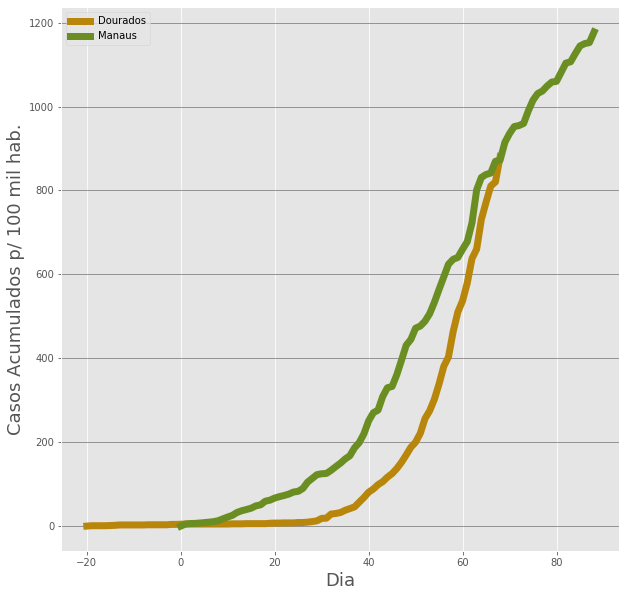
\includegraphics[width=.6\textwidth]{figs/Dourados_Manaus_casos.png}
  \caption{Curva do número de casos diagnosticados por 100 mil habitantes. Comparativo entre Dourados (MS) e Manaus (AM)}
  \label{fig:curva100K}
  \end{figure}

A maioria dos dados apresentados até então mostram um quadro estático, como um retrato de um momento da pandemia no estado do Mato Grosso do Sul. Para avaliar a evolução do quadro ao longo do tempo, produzimos a Figura~\ref{fig:curva100K}, em que se podem ver as curvas de casos por 100 mil habitantes por dia. Já a Figura~\ref{fig:curva100KLog} apresenta o número de casos por 100 mil habitantes em escala logarítmica (base 10) por dia. As Figuras~\ref{fig:curva100K} e \ref{fig:curva100KLog} apresentam a curva da cidade de Dourados comparada à curva de Manaus.

\begin{figure}[!htb]
  \centering
  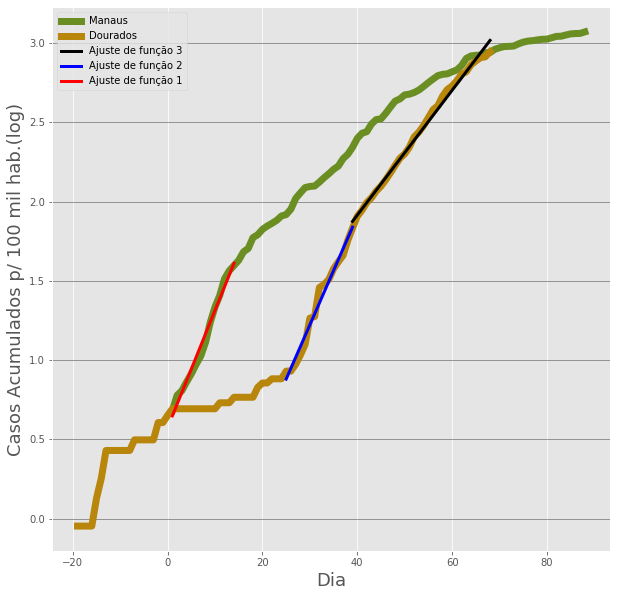
\includegraphics[width=.6\textwidth]{figs/Dourados_Manaus_casos_log.png}
  \caption{Curva do número de casos diagnosticados por 100 mil habitantes. Comparativo entre Dourados (MS) e Manaus (AM) em escala logarítmica (eixo y)}
  \label{fig:curva100KLog}
  \end{figure}

Na base de dados utilizada, o primeiro registro de casos em Manaus é do dia 28/03/2020, apresentando 105 casos. Considerando a população estimada em 2.182.763 habitantes, obtemos uma taxa de 4.81 casos por cem mil habitantes. Já em Dourados, o índice próximo de 4.81 casos por 100 mil habitantes só foi alcançado no dia 14/04/2020.

Para efeito de visualização de dados, o dia zero da curva de Dourados foi lançado nas Figuras~\ref{fig:curva100K} e \ref{fig:curva100KLog} na data em a cidade objeto deste estudo alcança a marca inicial do índice de casos por 100 mil habitantes de Manaus. O Amazonas foi um dos primeiros estados brasileiros a apresentar casos do novo corona vírus e a evolução até a marca de 4.81 casos por 100 mil habitantes
não foi registrado pela base de dados utilizada nessa análise. 

No começo da série temporal, a cidade de Manaus apresenta evolução com velocidade mais acentuada que Dourados (ajuste de função 1). Próximo ao ponto de arrefecimento da curva da capital do Amazona, a evolução da cidade de Dourados começa a apresentar velocidade crescente (ajuste de função 2) com inclinação próxima à registrada anteriormente em Manaus, por tempo também semelhante. Após um ligeiro arrefecimento, a velocidade da curva que indica os dos casos de contaminação de Dourados segue sem sinais fortesde mudança de padrão (ajuste de função 3). Na Figura~\ref{fig:curva100K}, é possível identificar que as curvas de casos por 100 mil habitante se aproximam e, na Figura~\ref{fig:curva100KLog} as curvas que mostram a velocidade da contaminação também se aproximam, considerando os critérios apresentados.

A comparação entre casos de estudo e casos emblemáticos da pandemia contribui para antecipar cenários futuros, embora toda ferramenta analítica apresente limitações. Um modelo matemático preditivo foi utilizado como um elemento adicional para nossa avaliação.

\section{Modelo Preditivo}


A busca de modelos matemáticos que pudessem ajudar a quantificar e estudar a evolução de epidemias não é um assunto novo. O primeiro modelo de sucesso data de 1927 (Kermack e McKendrick)\cite{doi:10.1098/rspa.1927.0118}. Ao longo do tempo, este modelo recebeu releituras e complementações que dão origem aos novos modelos aplicados em estudo de viroses e mais recentemente aplicados a previsões na pandemia da Covid-19. 

Hoje temos duas linhas bem distintas de modelos matemáticos aplicados à epidemiologia, os modelos estocásticos e os modelos determinísticos. Os modelos estocásticos usam regressões e séries temporais e as previsões são feitas com base em distribuições estatísticas. Um exemplo dessa classe é o modelo do grupo do \textit{Imperial College COVID-19 Response Team}\cite{impirial1}. O modelo DELPHI\cite{delphi} se encaixa na classe dos modelos determinísticos, em que um conjunto de equações diferenciais é integrado num problema de valor de contorno\cite{2008elementary}. 

O modelo DELPHI usa o conjunto de equações diferenciais conhecidas como $SEIRD$ onde as variáveis  são 
\begin{itemize}
\item $S$ para suscetível,
\item $E$ para exposto,
\item $I$ para infectados,
\item $R$ para recuperados,
\item $D$ para óbitos.
\end{itemize}
Este conjunto é organizado da seguinte forma ,

\begin{align*}
 \frac{dS}{dt} & = - \alpha \gamma(t) S(t) I(t) \\
 \frac{dE}{dt} & = \alpha \gamma(t) S(t) I(t) \\
 \frac{dI}{dt} & = r_i E(t) - r_d I(t) \\
 \frac{d AR}{dt} & = r_d(1 - p_{dth})(1 - p_d) I(t) - r_{ri} AR(t) \\
 \frac{d DHR}{dt} & =  r_d (1 - p_{dth}) p_d p_h I(t) - r_{rh} DHR(t) \\
 \frac{d DQR}{dt} & = r_d (1 - p_{dth}) p_d (1 - p_h) I(t) - r_{ri} DQR(t) \\
 \frac{d AD}{dt} & =  r_d p_{dth} (1 - p_d) I(t) - r_{dth} AD(t) \\
 \frac{d DHD}{dt} & =  r_d p_{dth} p_{dph} I(t) - r_{dth} DHD(t) \\
 \frac{d DQD}{dt} & =  r_d p_{dth} p_d(1 - p_h) I(t) - r_{dth} DQD(t) \\
 \frac{d TH}{dt} & = r_d p_d p_h I(t)  \\
 \frac{d DD}{dt} & =  r_{dth} (DHD(t) + DQD(t)) \\
 \frac{d DT}{dt} & = r_d  p_d I(t) \\
 \frac{d R}{dt} & =  r_{ri} (AR(t) + DQR(t)) + r_{rh} DHR(t) \\
 \frac{d D}{dt} & =  r_{dth} (AD(t) + DQD(t) + DHD(t)) \, .
\end{align*}

Além das variáveis $SEIRD$ tradicionais descritas acima, o modelo apresenta o detalhamento: 
\begin{itemize}
\item Não detectados $(AR)$ \& $(AD)$: pessoas infectadas e em auto quarentena em casa devido a efeitos da doença. São variáveis para tratar casos não detectados. De alguma maneira, as pessoas se recuperam $(AR)$ e algumas morrem  $(AD)$.

\item Detectados Hospitalizados $(DHR)$ \& $(DHD)$: pessoas infectadas e testadas que necessitaram de hospitalização. Novamente a terminação R para recuperados e D para mortos.

\item Detectados em quarentena $(DQR)$ \& $(DQD)$: pessoas infectadas e em quarentena em casa. Segue a designação de $R$ e $D$.

\end{itemize}

A primeira equação do conjunto representa que a variação do número de pessoas suscetíveis ao longo do tempo cai (sinal negativo) com a taxa de infecção $\alpha$ a função auxiliar $\gamma$ e o contato entre os suscetíveis $S$ e os infectados $I$. Da mesma forma, a segunda equação representa que o número de expostos aumenta com o contato entre os suscetíveis $S$ e os infectados $I$. Para a equação dos infectados, a terceira, temos que seu número aumenta com o tempo na taxa $r_i$ com a qual os expostos $E$ se tornam doentes, e cai com a taxa $r_d$. Assim, cada uma das equações seguintes representam como cada variável aumenta com a sua respectiva taxa de variação.  Na última equação, o total de óbitos é a soma dos possíveis caminhos previstos no modelo.


Os parâmetros do modelo são:
\begin{itemize}
 \item $\alpha$ taxa de infecção (ajustado).
 
 \item $\gamma(t)$ medidas governamentais e respostas:
\[
  \gamma(t) = \frac{2}{\pi} \arctan \left( \frac{-(t - a)}{b}  \right) + 1
\]
usando os  a and b, é possível modelar o tempo de duração dos ajustes como restrição de comércio, distanciamento social, etc. Os parâmetros $a$ e $b$ são ajustados.

\item $r_d$ é a taxa de detecção.   $ r_d = \frac{log 2}{T_d}$,
 onde $T_d$ é a mediana do tempo para detecção (suposto ser 2 dias). Parâmetro fixo.

\item $r_i$ é a taxa de infecção deixando o tempo de incubação. 
  $r_i = \frac{log 2}{T_i}$  onde $T_i$ é o tempo mediano para deixar o período de incubação (suposto ser 5 dias).  Parâmetro fixo.

\item $r_{ri}$ é taxa de recuperação fora da hospitalização. 
   $r_{ri} = \frac{log 2}{T_{ri}}$, onde $T_{ri}$ é a mediana do tempo de recuperação dos casos não hospitalizados (suposto ser 10 dias). Parâmetro fixo.

\item $r_{rh}$ é taxa de recuperação sob hospitalização.
$r_{rh} = \frac{log 2}{T_{rh}}$ where $T_{rh}$, é a mediana do tempo de recuperação dos casos  hospitalizados (suposto ser 15 dias). Parâmetro fixo.

\item $r_{dth}$ é a taxa de morte.
 $r_{dth} = \frac{log 2}{T_{dth}}$, onde $T_{dth}$ é o tempo de espera do paciente até a morte. Parâmetro ajustado aos dados históricos.

\item $p_{dth}$ é a taxa de mortalidade. Parâmetro ajustado diretamente das curvas de óbitos.

\item $p_d$ é a porcentagem de casos detectados. Este valor é fixo em 0.2. Isto significa que para cada caso conhecido há 5 casos não detectados. 

\item $p_h$ é a porcentagem de detectados hospitalizados. Também é constante. 

\end{itemize}


Antes de passarmos para as previsões do modelo é importante entender a ação da função $\gamma(t)$ na modelagem. A interpretação correta dos resultados depende deste entendimento.
\begin{figure}[t]
 \centering
 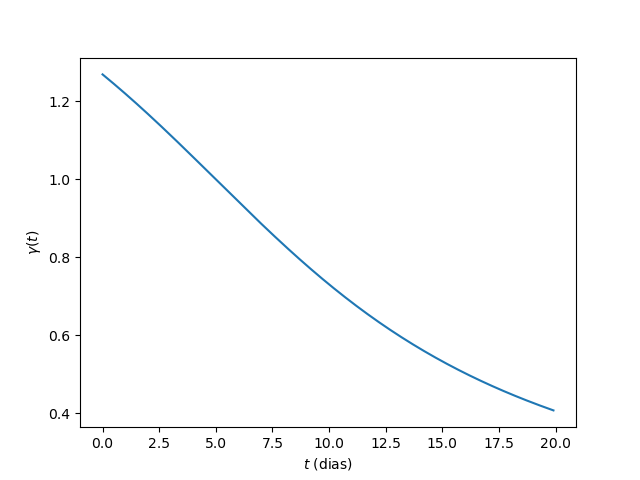
\includegraphics[width = 8cm]{figs/gamma_1.png}
 \caption{Formato típico da função $\gamma (t)$, aqui para os parâmetros $a = 20$ e $b = 5$. No processo de previsão estes números são ajustados.}
 \label{gamma}
\end{figure}


Na lista acima há parâmetros fixos e parâmetros ajustados. Os parâmetros fixos são aqueles que estão ligados à natureza humana, como tempo de incubação por exemplo, e não dependem de condições regionais. Os parâmetros ajustados são aqueles que vão carregar para o modelo as peculiaridades de cada população. O ajuste é feito com base nas curvas de óbitos acumulados (com peso maior) e nas curvas casos acumulados. O modelo considera o período a partir do centésimo caso acumulado detectado até a última atualização. O ajuste dos parâmetros é feito de forma a minimizar o quadrado da diferença entre a previsão o os casos reais. Os dados aqui usados são do Ministério da Saúde do Brasil \cite{minsaude}.  

\begin{figure}[t]
 \centering
 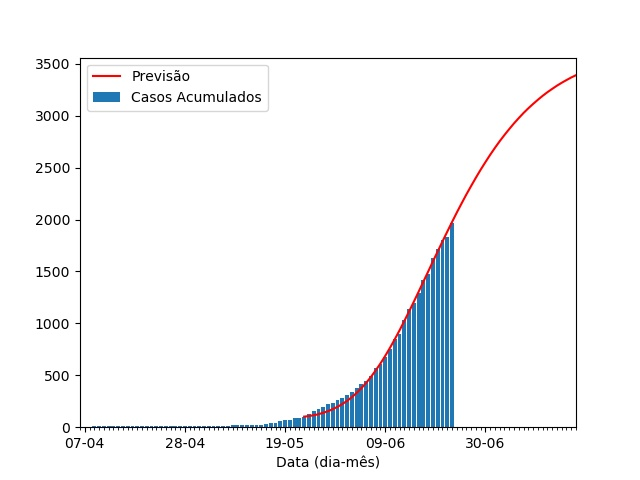
\includegraphics[width = 8cm]{figs/Fig_Brasil_MS_Dourados_casos_20200624_025dias.jpg}
 \caption{As barras azuis são número total de casos acumulados segundo o Ministério da Saúde para a cidade de Dourados - MS, e em vermelho a curva de previsão do modelo DELPHI para 25 dias.}
 \label{proj_casos}
\end{figure}


\begin{figure}[t]
 \centering
 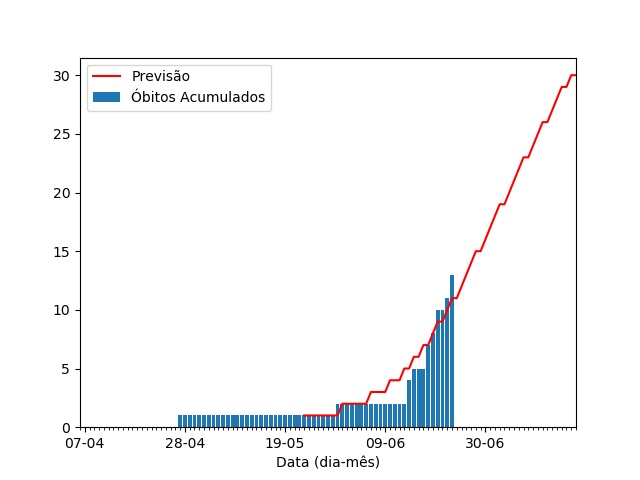
\includegraphics[width=8cm]{figs/Fig_Brasil_MS_Dourados_obitos_20200624_025dias.jpg}
 \caption{Gráfico de óbitos. Barras azuis são casos acumulados e curva vermelha previsão do modelo DELPHI para 25 dias.}
 \label{proj_obitos}
\end{figure}

Observando a Figura~\ref{gamma}, vemos que a função $\gamma(t)$ é sempre decrescente. Este fato captura o comportamento típico de uma epidemia viral onde a taxa de reprodução da doença normalmente cai com o número de infectados se tornando imunes ao longo do tempo, mas ela não é perfeita para a Covid-19. A adoção de medidas de isolamento social de fato contribui para a diminuição da taxa de reprodução e a função $\gamma$ como está é perfeita, porém a saída precoce do isolamento social pode fazer a taxa de reprodução voltar a crescer, e, nesse caso, a função necessita de ajuste, ou as previsões ficariam com tendência otimista. No modelo original, o grupo responsável pelo seu desenvolvimento acrescentou um módulo contando com as políticas adotadas em cada localidade. Esta implantação é restrita aos EUA, e não se aplica ao Brasil. Está em andamento um trabalho ainda inconcluso de adaptação desta estrutura de cálculo para o Brasil. Então, as previsões aqui apresentadas podem ter um viés otimista. 


A projeção, Figuras \ref{proj_casos} e \ref{proj_obitos}, aponta um aumento tanto no número de casos novos como no número de óbitos nos próximos dias. No ajuste dos parâmetros o modelo usa todos os dados do período a partir do dia do centésimo caso. Então, esta projeção é um apanhado de tudo que aconteceu anteriormente até o dia da último boletim. Para Dourados, o dia inicial é 23/5/2020 e o último boletim tem dados de 23/06/2020. O ajuste do modelo para ficou em acordo com casos reais neste período medido.

O comportamento social geral bem como a adoção ou ausência de medidas governamentais ficam embutidos nos parâmetros. O modelo permite previsões por quantos dias quisermos. Para a análise, foi escolhido um período de 25 dias para dar uma ideia do que acontece se nada mudar. Alterações do comportamento social atual podem alterar o padrão das curvas de crescimento, casos e óbitos, tanto para cima sem isolamento social, como para baixo com o isolamento  e consequentemente as respostas do modelo em rodadas futuras acompanharão estas mudanças.

Na Figura \ref{proj_casos} observamos que o comportamento de crescimento até hoje é exponencial. O mesmo comportamento vai se refletir na curva de óbitos, Figura \ref{proj_obitos}, que vinha mostrando um crescimento lento no número de mortes até 14/06/2020, e a partir daí dispara exponencialmente. Mantida esta tendência o número de óbitos pode dobrar em duas semanas.   

\section{Conclusão}\label{conc}

As previsões oferecidas pelo modelo, além dos dados reais, mostram um cenário de crescimento da pandemia em Dourados para as próximas semanas. Esta previsão leva em conta tudo que aconteceu a partir de 23/05/2020 até 23/06/2020, incluindo os cuidados e/ou a ausência deles ao longo do tempo. A forma mais eficiente conhecida para conter esta evolução é o distanciamento social. Continuaremos a fazer previsões e verificar o comportamento dessas tendências.

Segundo os dados analisados e a metodologia aplicada, nota-se uma importância do município de Dourados, tanto do ponto de vista dos casos absolutos, quanto do ponto de vista dos casos relativos e quanto da centralidade espacial em relação a outros municípios que apresentam números relevantes para serem levados em conta no planejamento das estratégias de combate ao vírus.

O objetivo de uma análise de dados é nortear as ações de técnicos, epidemiologistas, profissionais de saúde e gestores no enfrentamento à crise sanitária que estamos vivenciando. Mesmo com as limitações inerentes a cada ferramenta utilizada nesta pesquisa, a sobreposição de evidências permite recomendar extrema cautela na definição dos próximos passos. 


\bibliographystyle{sbc}
\bibliography{modelo.bib}

\end{document}
